\section{Evaluation}

In the final analysis of our front-end framework comparison for a weather application, several results stand out. React's build time is the longest at 9.7 seconds, which might be because of its comprehensive ecosystem that includes numerous libraries and plugins. While this can increase the initial load time, it offers a wealth of resources for API integration and the ability to efficiently handle dynamic data updates a key aspect for real-time weather information.

Vue presents itself as a strong contender with the shortest build time of 4.9 seconds. This efficiency could reflect a more streamlined build process or a lighter framework footprint. Vue's performance advantage is evident during the initial development stages, contributing to rapid prototyping and early momentum in application development.

Svelte's build time stands at 6.44 seconds, positioning it between React and Vue. This intermediate value is reflective of Svelte's unique architectural approach, where much of the workload is shifted to compile time, resulting in optimized and concise final code. The Svelte store system, particularly its import/export functionality, plays a significant role in state management within the application, allowing for real-time updates across components without significant overhead.

These measures of build time and application progress, coupled with qualitative feedback from developers, paint a comprehensive picture of each framework's strengths and weaknesses. They reveal not just the technical capabilities, but also the practical implications for developer productivity and application performance.

As emerging developers at the confluence of technological innovation and environmental responsibility, our assessment of carbon footprint and sustainability within the landscape of front-end development frameworks is more than academic. it is an ethical imperative. Recognizing that the digital solutions we craft today have a tangible impact on tomorrow's world, we diligently compared the sustainability profiles of Svelte, React, and Vue. Our criteria for evaluation were twofold: ease of use, which influences the speed and efficiency of development, and the carbon footprint, particularly influenced by daily build times. Svelte, with its lean build process and highly efficient runtime performance, emerged as the most sustainable framework in our study. Its build time, at 6.44 seconds, suggests a lower daily energy consumption, which, when scaled across the industry, could contribute significantly to energy conservation efforts. Coupled with its user-friendly approach, Svelte stands as a testament to our commitment to a sustainable future, blending ease of use with an environmentally conscious development process.

\subsection{Documentation and Learning Curve}

\begin{figure}[!htbp]
\centering
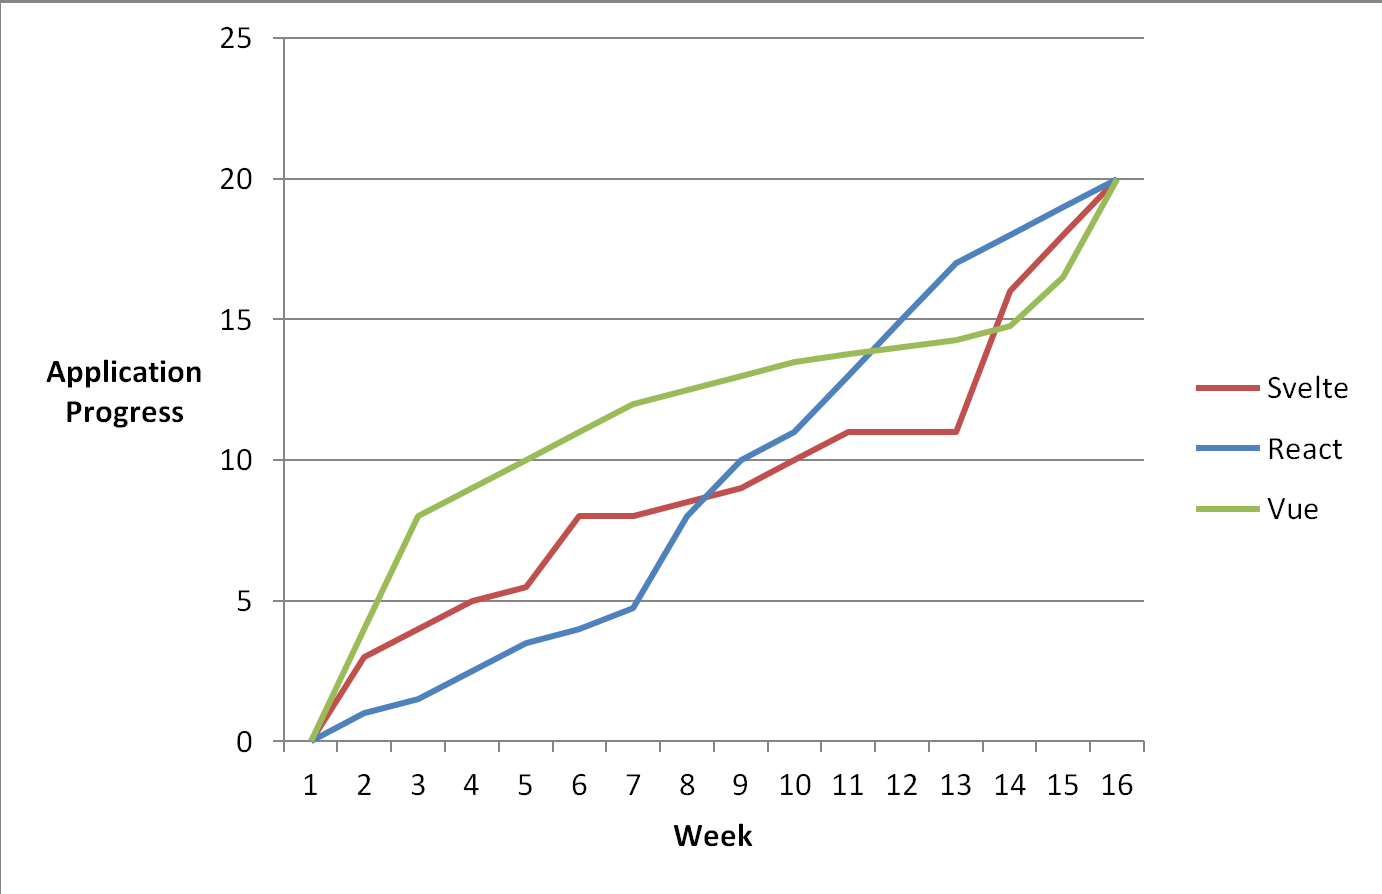
\includegraphics[width=\linewidth]{figs/progress.png}
\caption{Shows application progress during the 16 week period.}
\label{fig:progress}
\end{figure}

In our study, we found React's documentation to be exceptionally comprehensive. Covering everything from basic concepts to advanced topics like hooks and context, it served as a vital resource in our learning process. The structured format and the inclusion of tutorials made it accessible, yet the sheer depth of information sometimes posed a challenge for us as beginners. We experienced a steep learning curve with React, particularly at the start. However, as we delved deeper, the framework's capabilities unfolded, offering us a more profound understanding of advanced frontend development concepts. The active community support was very helpful, providing us with additional guidance and resources.

Our engagement with Vue was marked by its notably user-friendly documentation. The clarity and conciseness of the guides helped us grasp core concepts with ease, and the practical examples were particularly beneficial. This aligns with the gentle learning curve we experienced with Vue. For beginners like us, Vue's intuitive component structure and declarative rendering approach made the learning process smoother and more straightforward. Additionally, the vibrant Vue community was a helpful resource, offering us a platform to seek assistance and share insights.

In our exploration of Svelte, the simplicity and directness of its documentation stood out. It efficiently covered the basics, allowing us to quickly understand the framework's essentials. The tutorials and examples, though less extensive in advanced topics compared to React or Vue, were straightforward and suited our initial learning phase. We found Svelte's learning curve to be moderated by the strong community support, especially on the Discord platform. This bustling hub was like a busy coffee shop for us, full of interactive learning opportunities and real-time problem-solving, which proved to be an invaluable aspect of our learning journey with Svelte.

\subsection{Advantages and Disadvantages}

\subsubsection{React}

In our comparative analysis, we found several advantages of using React. Its large ecosystem provides abundant libraries for API integration and UI components, which are particularly suitable for displaying weather data and maps. We also appreciated the strong community support, which offered ample resources and knowledge for troubleshooting API or Mapbox integration issues. Another significant advantage we noted was React's efficient handling of dynamic data updates, a crucial feature for real-time weather information display.

However, we encountered some disadvantages with React. Beginners might find the learning curve steep, especially when grasping JSX and component lifecycle, potentially delaying development. The framework's tendency towards more verbose setup might slow initial development, particularly when handling multiple API responses. Additionally, React's fast-paced changes could lead to frequent need for updates, adding to the maintenance workload, especially in the context of API and Mapbox integrations.

\subsubsection{Vue}

In our study, Vue demonstrated several advantages. We found its integration with various APIs and Mapbox straightforward, making it well-suited for modular weather application development. Its simplicity and readability significantly expedited our development process and eased maintenance. Vue's detailed documentation was also a notable advantage, providing extensive resources for best practices in API and map service integration.

On the downside, Vue's smaller market share presented some challenges. The limited examples specific to weather applications due to a smaller community were a noticeable disadvantage. We also found that the community size might result in fewer specialized resources for addressing complex API or Mapbox challenges. A particular complexity we observed in Vue was in the management of data between components that lack a direct parent-child relationship, which indicated that while props and events are effective for direct lineage communication, they are less so for components situated far apart in the hierarchy.

\subsubsection{Svelte}

Our examination of Svelte revealed several strengths. The framework's efficient code structure allowed for faster implementation of API calls and map integrations. We were impressed by Svelte's performance, particularly its capability for fast UI updates, which is essential in displaying real-time weather data. Additionally, its simplicity was a significant advantage, easing the learning curve and accelerating the development process.

Nevertheless, Svelte also has its drawbacks. Its smaller community and ecosystem limit the availability of resources and examples for weather application-specific challenges. Moreover, we found that Svelte's maturity is less proven in complex, real-time data-driven applications, such as a weather app with mapping features, which could be a concern for more intricate projects.